\section{Сингулярное разложение.}

\begin{statement}
  Пусть $A\in\R^{m\times n}$, $m\geq n$. Тогда справедливо \textit{сингулярное} разложение
  \[A=U\Sigma V^T=(U_1U_2)\left(\begin{array}{c}
        \Sigma_n \\ 0
      \end{array}\right)V^T\]
  \begin{itemize}
    \item $U\in\R^{m\times m}=(\mathbf{u}_1,\ldots,\mathbf{u}_m)$ - ортогональная матрица \textit{левых сингулярных векторов}, $U_1\in\R^{m\times n}$, $U_2\in\R^{m\times (m-n)}$
    \item $V\in\R^{n\times n}=(\mathbf{v}_1,\ldots,\mathbf{v}_n)$ - ортогональная матрица \textit{правых сингулярных векторов}.
    \item $\Sigma_n\in\R^{n\times n}$ - диагональная матрица,
          на диагонали которой расположены упорядоченные \textit{сингулярные числа} $\sigma_1\geq\sigma_2\geq\ldots\sigma_n\geq0$.
  \end{itemize}
\end{statement}

Если $m = n$, то $\Sigma=\Sigma_n$.

Построив $SVD$-разложение можно установить, является ли задача вырожденной
($\sigma_n=0$), невырожденной ($\sigma_n\neq0$), `хорошей' ($\sigma_1/\sigma_n$ не слишком велико).

Если $m<n$; то сингулярное разложение строят для матрицы $A^T$.
Если $A=A^T$, то сингулярные числа $\sigma_{i}=\abs{\lambda_i(A)}$,
т.е. с точностью до знака совпадают с собственными числами,
сингулярные векторы $\mathbf{v}_i$ являются соответствующими собственными векторами.
В случае, если $\lambda_i(A)<0$, то минус утаскивают в соответствующий
вектор в $U$, и поэтому разложение возможно.

Как найти $U$ и $V$? Рассмотрим следующие выражения
\[AA^T=U\Sigma V^T(U\Sigma V^T)^T=U\Sigma V^TV^T\Sigma^T U^T=U\Sigma_n^2U^T\]
\[A^TA=(U\Sigma V^T)^TU\Sigma V^T=V\Sigma U^TU\Sigma^T V^T=V\Sigma_n^2V^T\]
Таким образом, $U$ и $V$ состоят из собственных
векторов для матрицы $AA^T\in\R^{m\times m}$ и $A^TA\in\R^{n\times n}$ соответственно,
которые для данных симметричных матриц являются ортогональными.
Такие вектора можно найти с помощью разложения матрицы в Жорданову форму.

\textbf{Геометрическая интерпретация SVD-разложения}.

Рассмотрим оператор $A$, переводящий элемент $\mathbf{x}\in\R^n$ в элемент $\mathbf{y}\in\R^m$.
Единичная сфера из $\R^n$ под действием $A$ переходит в
эллипсоид в подпространстве $\text{span}<\mathbf{u}_1,\ldots,\mathbf{u}_n>\subset\R^m$.
Вектора $\mathbf{u}_i$ задают полуоси эллипсоида,
$\mathbf{v}_i$ их прообразы, $\sigma_i$ коэффициенты удлинения векторов $\mathbf{v}_i$.

\[U\Sigma V^T\left(
  \tikzsetnextfilename{28/SVDBase}
  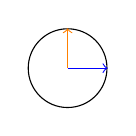
\begin{tikzpicture}[baseline=(current bounding box.center)]
    \node[draw,circle,minimum size=1cm] (c) at (0,0){};
    \draw[color=blue, ->] (0,0) -- (c.east);
    \draw[color=orange, ->] (0,0) -- (c.north);
  \end{tikzpicture}
  \right)\rightarrow
  U\Sigma\left(
  \tikzsetnextfilename{28/SVDScaledInRn}
  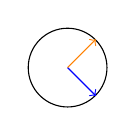
\begin{tikzpicture}[baseline=(current bounding box.center)]
    \node[draw,circle,minimum size=1cm] (c) at (0,0){};
    \draw[color=blue, ->] (0,0) -- (c.south east);
    \draw[color=orange, ->] (0,0) -- (c.north east);
  \end{tikzpicture}
  \right)\rightarrow
  U\left(
  \tikzsetnextfilename{28/SVDStretchedInRn}
  \begin{tikzpicture}[baseline=(current bounding box.center)]
    \node[draw,ellipse, minimum width = 1.8cm, minimum height = 1.2cm] (c) at (0,0){};
    \draw[color=blue, ->] (0,0) -- (c.south east);
    \draw[color=orange, ->] (0,0) -- (c.north east);
  \end{tikzpicture}\right)\rightarrow
  \tikzsetnextfilename{28/SVDScaledInRm}
  \begin{tikzpicture}[baseline=(current bounding box.center)]
    \node[draw,ellipse, minimum width = 1.8cm, minimum height = 1.2cm,rotate=40] (c) at (0,0){};
    \draw[color=blue, ->] (0,0) -- (c.south east);
    \draw[color=orange, ->] (0,0) -- (c.north east);
  \end{tikzpicture}
\]

\textbf{Алгебраическая интерпретация SVD-разложения}.
Рассмотрим оператор $A$, переводящий элемент $\mathbf{x}\in\R^n$ в элемент $\mathbf{y}\in\R^m$.
В пространстве $\R^n$ $\exists$ ортонормальный базис $\mathbf{v}_i$,
а в пространстве $\R^m$ - ортонормальный базис $\mathbf{v}_j$.
Тогда для произвольного $\mathbf{x}\in\R^n$:
\[A\mathbf{x}=U\Sigma V^T\mathbf{x}=U\Sigma V^T\sum_{i=1}^n\alpha_i\mathbf{v}_i=U\Sigma \sum_{i=1}^n\alpha_i\mathbf{e}_i=U\sum_{i=1}^n\sigma_i\alpha_i\mathbf{e}_i=\sum_{i=1}^n\sigma_i\alpha_i\mathbf{u}_i\]
А вектора $\mathbf{u}_{n+1},\ldots,\mathbf{u}_m$ добавляются как ортонормальное
добавление к векторам $\mathbf{u}_1,\ldots,\mathbf{u}_n$ для соблюдения $U^TU=I$.

% Теорема о наилучшем приближении матрицы малоранговыми матрицами в норме, подчиненной евклидовой.
% Не вошла в программу
